\documentclass[aspectratio=169, 8pt,t]{beamer}
\graphicspath{{figures/}} % Setting the graphicspath

% Theme settings
\usetheme{Madrid}
\usecolortheme{default}
\setbeamertemplate{navigation symbols}{}   % removes navigation symbols such as 'next page'
\setbeamertemplate{footline}{}             % remove line with name, date, page nr. 
\setbeamercolor*{frametitle}{bg=white}     % remove background from frametitle
\usepackage{caption}
% \captionsetup[figure]{labelformat=empty}% redefines the caption setup of the figures environment in the beamer class.
\setbeamersize{text margin left=20pt,text margin right=10pt}
\usefonttheme[onlymath]{serif} % makes beamer math look like article math
\usepackage{hyperref}


%======================= page numbering =======================
\addtobeamertemplate{navigation symbols}{}{ \usebeamerfont{footline}
  \insertframenumber / \inserttotalframenumber \hspace*{2mm} \\ \vspace*{1mm} 
}


%=================================== colors ====================================
\definecolor{RoyBlue}{RGB}{22, 46, 69}
\definecolor{RoyGrey}{RGB}{64, 88, 128} 

\newcommand{\hlme}[1]{{\color{red}\bf #1}} % highlight me

\setbeamercolor{structure}{fg=RoyBlue} % itemize, enumerate, etc
\setbeamercolor{frametitle}{fg=RoyGrey}
\setbeamercolor{section in head/foot}{bg=RoyBlue}


%======================= add progress dots to headline =========================
\setbeamertemplate{headline}{%
    \begin{beamercolorbox}[ht=4mm,dp=4mm]{section in head/foot}
        \insertnavigation{\paperwidth}
    \end{beamercolorbox}%
}%
\makeatother


%======================= add section title page ================================
\AtBeginSection[]{
  \begin{frame}
  \vfill
  \centering
    \usebeamerfont{title}\insertsection\par%
  \vfill
  \end{frame}
}


%=================================== titlepage =================================
\title{Electroweak and QED effects in PDF determination}
\date{QCD@LHC 2023  \\[0.1cm] 4 September 2023, Durham}
\author{Roy Stegeman}
\institute{\small The University of Edinburgh}


\titlegraphic{\vspace*{6mm}
  
\includegraphics[height=1.5cm]{logos/edi_logo.png} \hspace{10mm}
  % 
\includegraphics[height=0.8cm]{logos/nnpdf_logo_official.pdf} \hspace{10mm}
  
\includegraphics[height=1.5cm]{logos/higgs_logo.jpg}
}

\defbeamertemplate{title page}{noinstitute}[1][]
{
  \vbox{}
  \vfill
  \begingroup
    \centering
    \begin{beamercolorbox}[sep=8pt,center,#1]{title}
      \usebeamerfont{title}\inserttitle\par%
      \ifx\insertsubtitle\@empty%
      \else%
        \vskip0.25em%
        {\usebeamerfont{subtitle}\usebeamercolor[fg]{subtitle}\insertsubtitle\par}%
      \fi%     
    \end{beamercolorbox}%
    \vskip2em\par
    \begin{beamercolorbox}[sep=0pt,center,#1]{author}
      \usebeamerfont{author}\insertauthor
    \end{beamercolorbox}
  \begin{beamercolorbox}[sep=0pt,center,#1]{author}
    \usebeamerfont{institute}\insertinstitute
  \end{beamercolorbox}
  \vspace*{8pt}
  \vspace*{16pt}
    \begin{beamercolorbox}[sep=0pt,center,#1]{date}
      \usebeamerfont{date}\insertdate
    \end{beamercolorbox}\vskip0.5em
    {\usebeamercolor[fg]{titlegraphic}\inserttitlegraphic\par}
  \endgroup
  \vfill
}

\makeatletter
\setbeamertemplate{title page}[noinstitute][colsep=-4bp,rounded=true,shadow=\beamer@themerounded@shadow]
\makeatother


\begin{document}
{
\setbeamertemplate{headline}{} % remove headline from titlepage
\begin{frame}
  \titlepage
\end{frame}
}

\setbeamertemplate{enumerate items}[default]

\pgfdeclarelayer{bg}    % declare background layer
\pgfsetlayers{bg,main}  % set the order of the layers (main is the standard layer)


% SLIDES =======================================================================


% Introduction:
%   - factorization
%   - status of modern PDFs: good agreement, approaching percent-level accuracy
%   - 3 necessary ingredients for the LHC precision era should be considered together: N3LO, theory uncertainty, QED

% aN3LO: % only discuss splitting functions in more detail
%   - Requirements: splitting functions, heavy-quark matching conditions, DIS coefficients, Hadronic coefficients (K-factors)
%   - Status of 4-loop splitting functions
%   - different approximation between NNPDF (with IHOU) and MSHTaN3LO (nuisance parameter), show comparison of splitting functions

% Theory uncertainties:
%   - IHOU for N3LO
%   - MHOU: scale variations are commonly used for partonic cross-sections -> use same idea to construct a covmat
%   - show plot comparing NNLO-NLO to MHOU, MHOU conservative
%   - impact of MHOU on PDF fit (show plots)
%   - compare aN3LO with IHOU&MHOU and NNLO with MHOU

% QED: % don't include discussion of DGLAP basis since that's too technical
%   - Requirements: splitting functions, photon PDF (luxQED), ideally photon initiated theory calculations
%   - discuss luxQED, modified momentum sumrule. 
%   - slightly different procedures (different initial scale choices): 
%     NNPDF: iterative procedure due to photon in MSR, 
%     MSHT20: PI contributions
%     CT18: own uncertainty estimation
%   - comparison plots: NNPDF4.0 vs NNPDF4.0QED, NNPDF4.0QED vs CT18qed vs MSHT20qed
%   - pheno plots form NNPDF4.0QED draft, high 
%   - (optional) highlight pineAPPL

% Summary and Outlook



\section*{Introduction}

% TODO: color DY schemetic corresponding to colors of equation
\begin{frame}{Factorization and universality}
  Collinear factorization enables the prediction of cross-sections
  \begin{equation*}
    \sigma_{\mathrm{LHC}}(M, s) \propto \sum_{i j} \int_{M^2}^s d \hat{s} {\color{blue}\mathcal{L}_{i j}(\hat{s}, s)} {\color{red}\hat{\sigma}_{i j}\left(\hat{s}, \alpha_s(M)\right)}, \quad i,j = \{g, u, \bar{u}, d, \bar{d}, \ldots\}
  \end{equation*}

  \begin{columns}
    \begin{column}{0.49\textwidth}
      Partonic luminosity
      \begin{equation*}
        {\color{blue}\mathcal{L}_{i j}(Q, s)}=\frac{1}{s} \int_{Q^2 / s}^1 \frac{d x}{x} {\color{teal}f_i\left(\frac{Q^2}{s x}, Q\right) f_j(x, Q)}
      \end{equation*}
      Parton Distribution Function:
      \begin{equation*}
        {\color{teal} f_j(x,Q)}
      \end{equation*}
      \begin{itemize}
        \item Non-perturbative QCD
        \item Extracted from experimental data
        \item Universal
      \end{itemize}
    \end{column}

    \begin{column}{0.49\textwidth}
      {\color{red} $\hat{\sigma}_{i j}\left(\hat{s}, \alpha_s(M)\right)$} denotes the hard-scattering coefficient function
      \begin{itemize}
        \item Calculable in perturbative QCD
        % \item infrared safe
        \item Independent of the initial hadron
      \end{itemize}
      \begin{figure}
        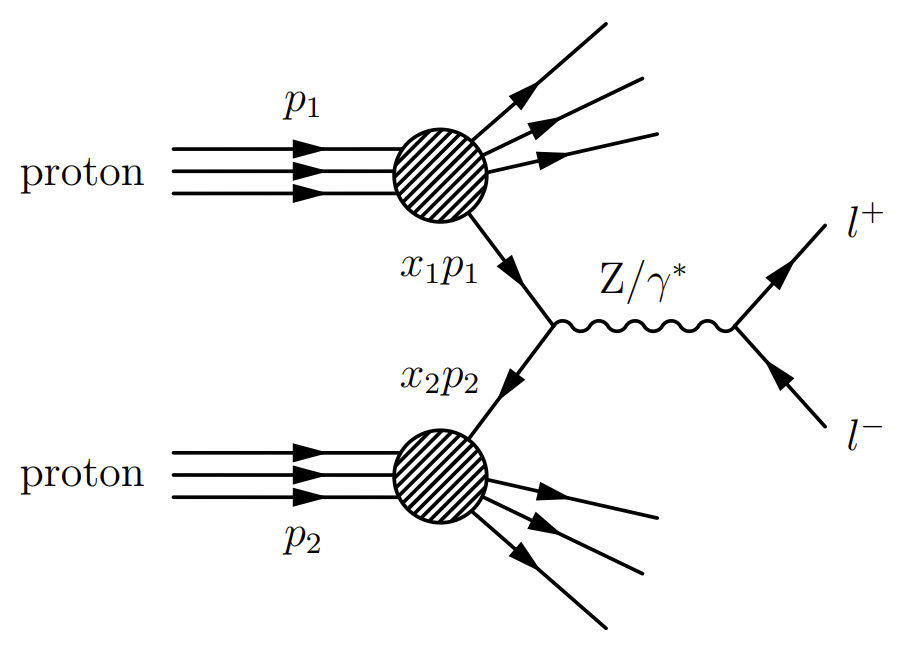
\includegraphics[width=0.5\textwidth]{figures/dy.png}
      \end{figure}
    \end{column}
  \end{columns}
\end{frame}



\begin{frame}{Status of modern PDF sets}
  PDF sets are provided by various collaborations, each using slightly different theory choices, datasets, and methodologies
  \begin{columns}
    \begin{column}{0.49\textwidth}
      \begin{figure}
        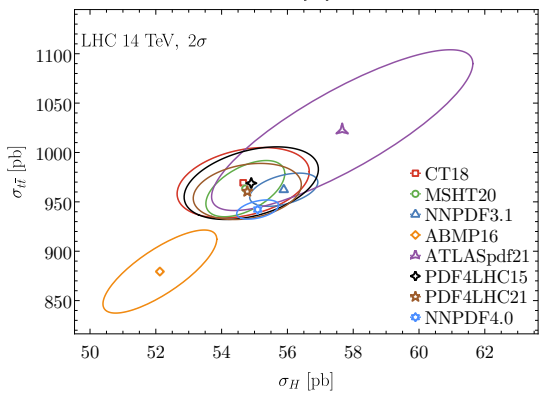
\includegraphics[width=0.6\textwidth]{figures/Httbar_xsec.png}
        \caption*{\color{gray}\small \footnotesize [Snowmass 2021: 2203.13923]}
      \end{figure}
    \end{column}
    \begin{column}{0.49\textwidth}
      \begin{figure}
        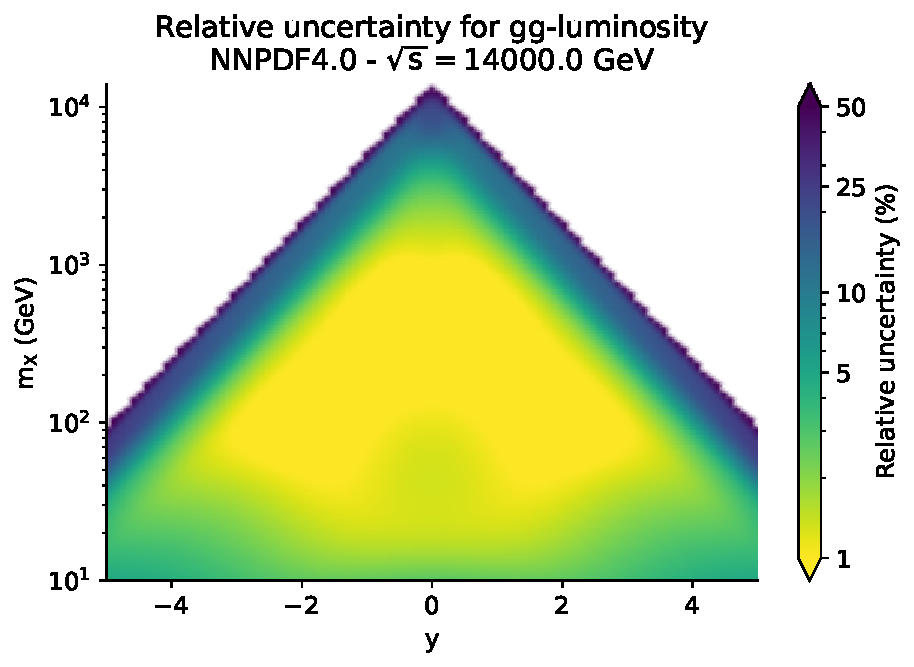
\includegraphics[width=0.6\textwidth]{figures/gglumi.pdf}
      \end{figure}
    \end{column}
  \end{columns}
  \begin{columns}
    \begin{column}{0.49\textwidth}
      \begin{itemize}
        \item Current standard is NNLO in QCD
        \item Results are generally consistent, but uncertainties differ
        \item Approaching percent-level accuracy
      \end{itemize}    
    \end{column}
    \begin{column}{0.49\textwidth}
      \begin{itemize}
        \item CT: Hessian + tolerance
        \item MSHT: Hessian + dynamic tolerance
        \item NNPDF: MC + closure tests
      \end{itemize}    
    \end{column}
  \end{columns}
\end{frame}


\begin{frame}{Challenges}
  PDFs, along with $\alpha_s$, are often a dominant source of uncertainty for predictions of LHC cross-sections 
  \begin{columns}
    \begin{column}{0.49\textwidth}
      \vspace*{1em}

      Requirements for the next generation of PDFs are threefold:
      \begin{itemize}
        \item To exploit the impressive progress in N3LO calculations we require PDFs of the same order
        \item Missing higher order uncertainties (MHOUs) for some observables are larger than the experimental uncertainty and can thus no longer be neglected
        \item The level of precision aimed for at the LHC no longer allows neglecting EW corrections
      \end{itemize}

      \vspace*{1em}
      Focus on QED, but first briefly mention N3LO and MHOU
    \end{column}

    \begin{column}{0.49\textwidth}
      \begin{figure}
        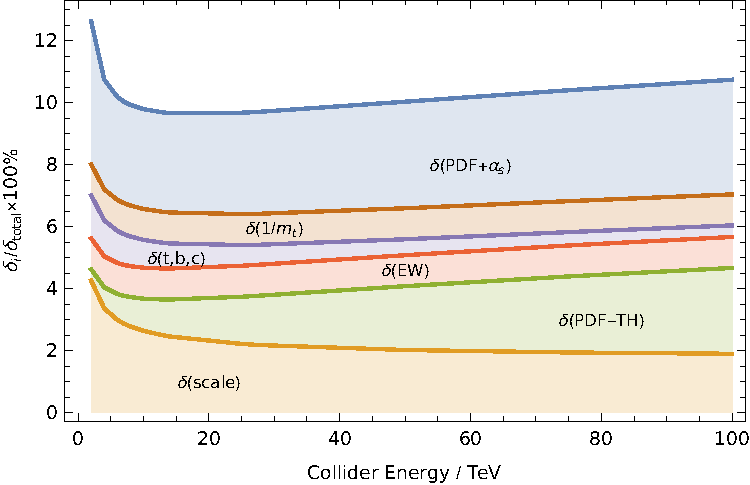
\includegraphics[width=0.8\textwidth]{figures/sources_of_unceratinty.pdf}
        \caption*{Uncertainties for inclusive Higgs production \\ 
        \color{gray}\small [HL-LHC: 1902.00134]}
      \end{figure}
    \end{column}
  \end{columns}
\end{frame}


% ==============================================N3LO===========================
\section{Approximate N3LO PDFs}

\begin{frame}{Towards N3LO PDFs}
  \begin{columns}[T]
    \begin{column}{0.59\textwidth}
      To produce PDFs at N3LO several inputs are needed at the corresponding order:
      \begin{itemize}
        \item QCD splitting functions for DGLAP evolution
        \item Matching conditions for heavy-quark mass schemes
        \item DIS partonic coefficients
        \item K-factors for hadronic observables
      \end{itemize}
    
      These are not completely available at N3LO
    
      \vspace*{1em}
      What do we know about 4-loop splitting functions?
      \begin{itemize}
        \item Singlet and Non-singlet Mellin Moments
        {\color{gray}\small [Davies, Falcioni, Herzog, Kom, Moch, Ruijl, Ueda, Vermaseren, Vogt: 1707.08315, 1610.07477, 2202.10362, 1610.0744, 2111.15561, 2302.07593, 2307.04158]}
        % \item Large-$n_f$ limits: {\color{gray}\small [Davies, Vogt, Ruijl, Ueda, Vermaseren: 1610.0744], [Falcioni, Herzog, Moch, Vogt: 2302.07593, 2307.04158], [Moch, Ruijl, Ueda, Vermaseren, Vogt: 2111.15561]}
        \item Small-x limits (BFKL resummation) {\color{gray}\small [Bonvini and Marzani: 1805.06460] [Davies, Kom, Moch, Vogt: 2202.10362]}
        \item Large-x limits (threshold resummation) {\color{gray}\small [Duhr, Mistlberger, Vita 2205.04493], [Henn, Korchemsky, Mistlberger: 1911.10174], [Soar, Moch, Vermaseren, Vogt: 0912.0369]}
      \end{itemize}
    \end{column}
    \begin{column}{0.39\textwidth}
      \begin{figure}
        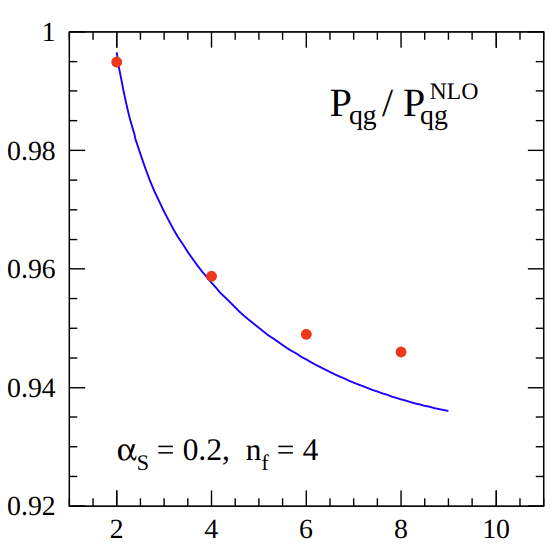
\includegraphics[width=0.8\textwidth]{figures/splittingmoments.png}
        \caption*{\color{gray}\small[Moch, Ruijl, Ueda, Vermaseren, Vogt: 2111.15561]}
      \end{figure}
    \end{column}
  \end{columns}


\end{frame}

\begin{frame}{Splitting functions at aN3LO}
  \begin{columns}[T]
    \begin{column}{0.49\textwidth}
      Splitting function approximation:
      \begin{itemize}
        \item Construction of approximate splitting function susceptible to  model uncertainties
        \item MSHTaN3LO posterior uncertainties based on fitting nuisance parameter {\color{gray}\small[McGowan, Cridge, Harland-Lang, Thorne: 2207.04739]}
        \item NNPDF4.0 accounts for model uncertainty through covariance matrix formalism
        \item Generally good agreement except for $P_{gq}$ where MSHT20aN3LO appears to saturate and deviates from NNLO
      \end{itemize}
    \end{column}
    \begin{column}{0.49\textwidth}
      \vspace*{-4em}
      \begin{figure}
        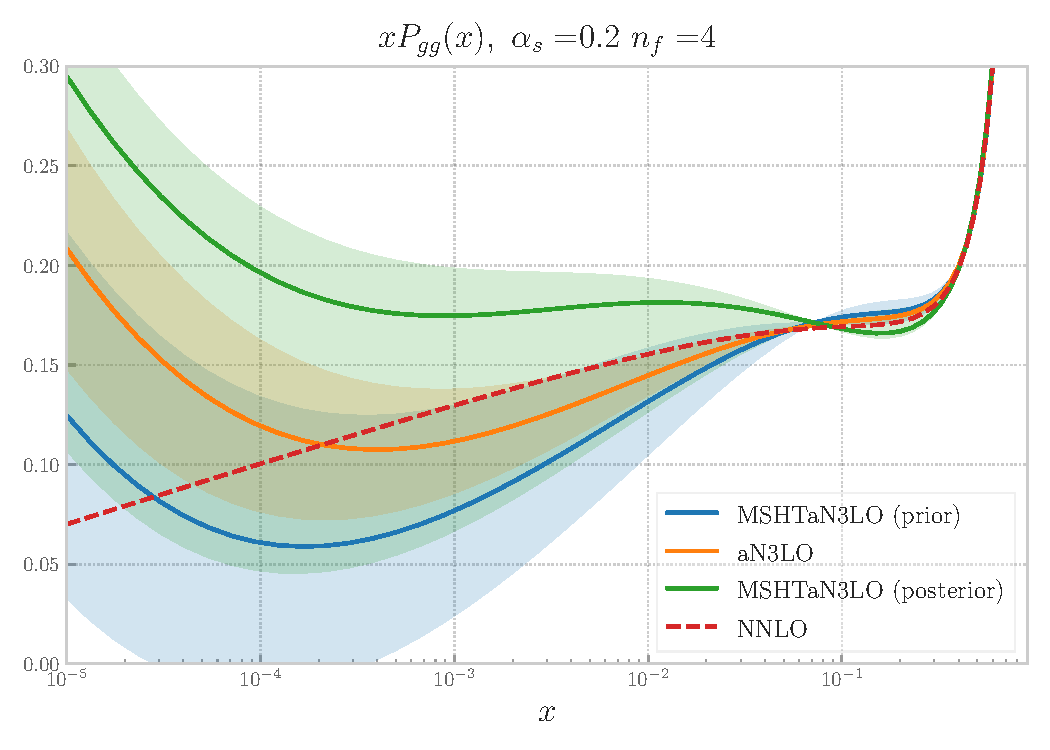
\includegraphics[width=0.65\textwidth]{figures/gamma_gg_msht_logx.pdf}\\
        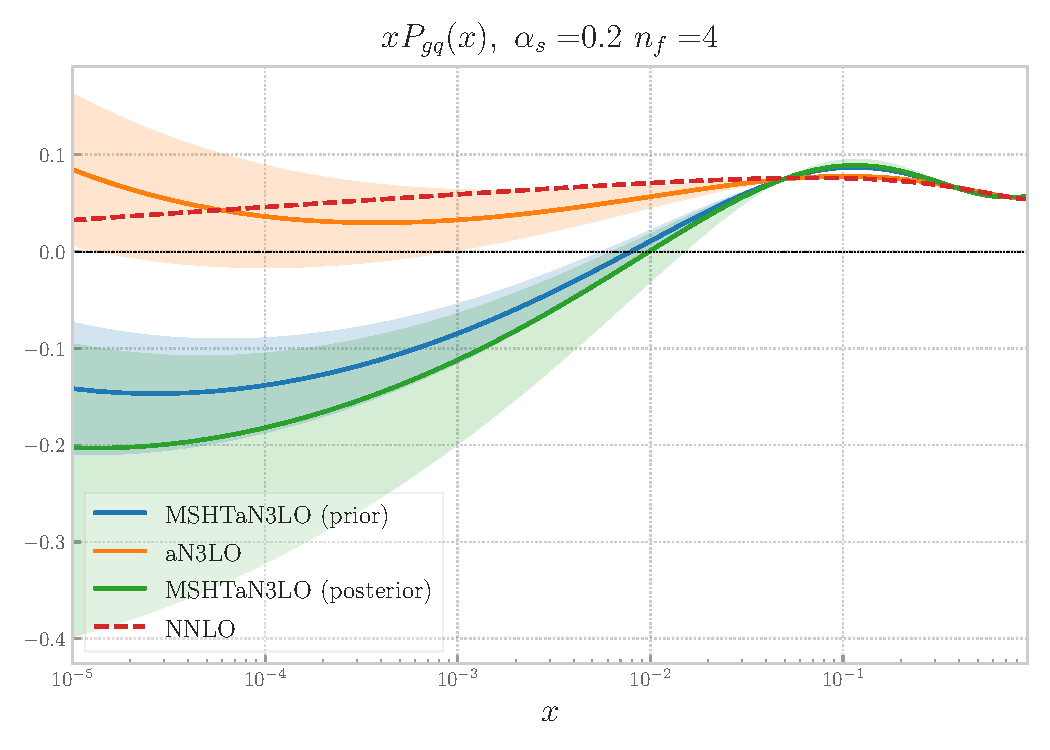
\includegraphics[width=0.65\textwidth]{figures/gamma_gq_msht_logx.pdf}
        \caption*{\color{gray}\small [NNPDF, Magni: 2023]}
      \end{figure}
    \end{column}
  \end{columns}
\end{frame}

% \begin{frame}{4-loop splitting functions}
%   The complete N3LO splitting functions are not yet know, but a lot of information is available:
%   \begin{itemize}
%     \item Non-singlet splitting functions are estimated to quite high precision \\
%     {\color{gray}\small [Moch, Ruijl, Ueda, Vermaseren, Vogt: 1707.08315], [Davies, Vogt, Ruijl, Ueda, Vermaseren: 1610.07477] [Davies, Kom, Moch, Vogt: 2202.10362] }
%     \item Singlet spitting functions are more challenging, main results used for approximation are:
%     \begin{itemize}
%       \item Large-$n_f$ limit: {\color{gray}\small [Davies, Vogt, Ruijl, Ueda, Vermaseren: 1610.0744]}
%       \item Small-x limit: {\color{gray}\small [Bonvini and Marzani: 1805.06460] [Davies, Kom, Moch, Vogt: 2202.10362]}
%       \item Large-x limit: {\color{gray}\small [Duhr, Mistlberger, Vita 2205.04493], [Henn, Korchemsky, Mistlberger: 1911.10174], [Soar, Moch, Vermaseren, Vogt: 0912.0369]}
%       \item Mellin Moments: {\color{gray}\small [Falcioni, Herzog, Moch, Vogt: 2302.07593, 2307.04158], [Moch, Ruijl, Ueda, Vermaseren, Vogt: 2111.15561]}
%     \end{itemize}
%   \end{itemize}

%   \begin{itemize}
%     \item Different functions can be used to combine known moments and results, this has a corresponding incomplete higher order uncertainty (IHOU)
%     \item So far only MSHTaN3LO is available, NNPDF4.0aN3LO coming soon!  
%   \end{itemize}
% \end{frame}


% \begin{frame}{Comparison of aN3LO splitting functions}
%   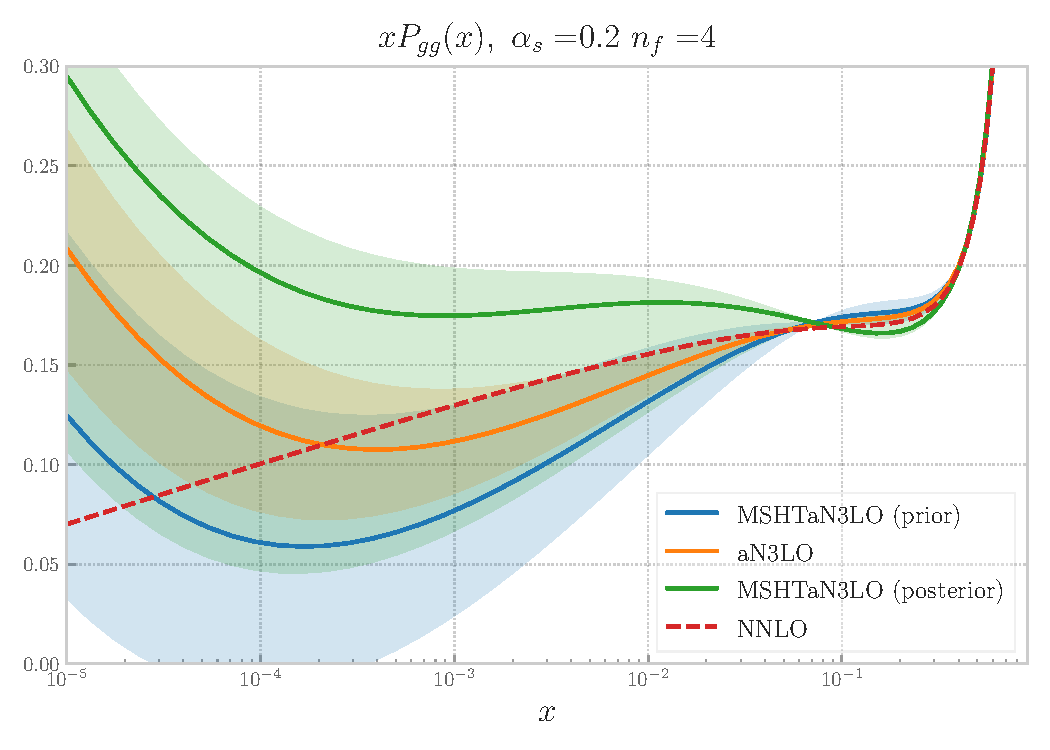
\includegraphics[width=0.39\textwidth]{figures/gamma_gg_msht_logx.pdf}
%   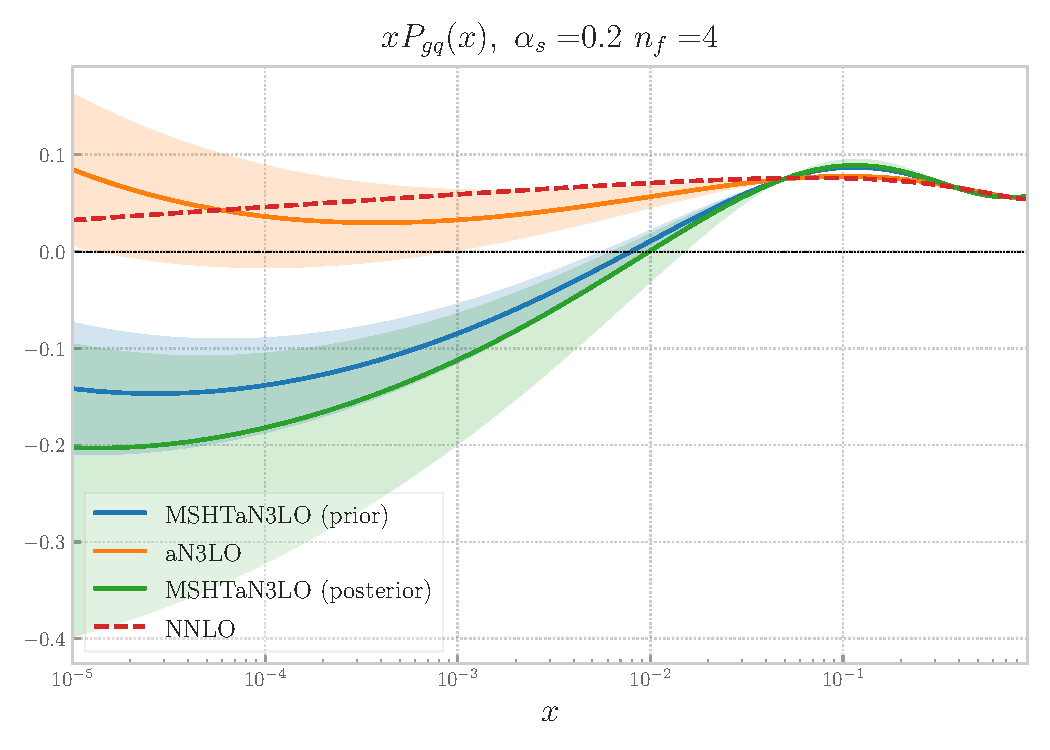
\includegraphics[width=0.39\textwidth]{figures/gamma_gq_msht_logx.pdf}
%   \begin{itemize}
%     \item MSHTaN3LO posterior uncertainties based on fitting nuisance parameter
%     \item To avoid fitting a nuisance parameter NNPDF4.0 accounts for IHOU through covariance matrix formalism
%     \item Generally good agreement except for $P_{gq}$
%   \end{itemize}
% \end{frame}


% ========================================Theory uncs===========================

\section{Missing higher order uncertainties}

\begin{frame}{Estimating missing higher order uncertainties}
  Unknown residual terms have a corresponding MHOU
  \begin{equation*}
    \hat{\sigma}\left(\alpha_s\right)=\hat{\sigma}^{(0)}\left(\sum_{k=0}^m \alpha_s^k\right)+\mathcal{O}\left(\alpha_s^{m+1}\right)
    \end{equation*}
  \begin{columns}[T]
    \begin{column}{0.49\textwidth}
      \begin{itemize}
        \item Commonly scale variations at N$^n$LO are used to estimate N$^{n+1}$LO MHOU
        \begin{itemize}
          \item factorization scale variation estimates MHOU in DGLAP evolution
          \item renormalization scale variation estimates MHOU in hard processes
        \end{itemize}
        \item MHOU PDFs have been determined using the theory covariance matrix formalism {\color{gray}\small [NNPDF: 1906.10698]}
        \begin{itemize}
          \item $\operatorfont{cov_{exp}} \rightarrow \operatorfont{cov_{exp}}+\operatorfont{cov_{theory}}$
        \end{itemize}
      \end{itemize}
    \end{column}
    \begin{column}{0.49\textwidth}
      \vspace*{-2em}
      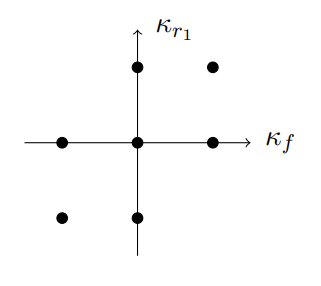
\includegraphics[width=0.89\textwidth]{figures/7ptsv.png}
    \end{column}
  \end{columns}
\end{frame}

\begin{frame}{Validating missing higher order uncertainties}
  Compare estimated MHOU at NLO to NNLO-NLO shift:
  \begin{figure}
    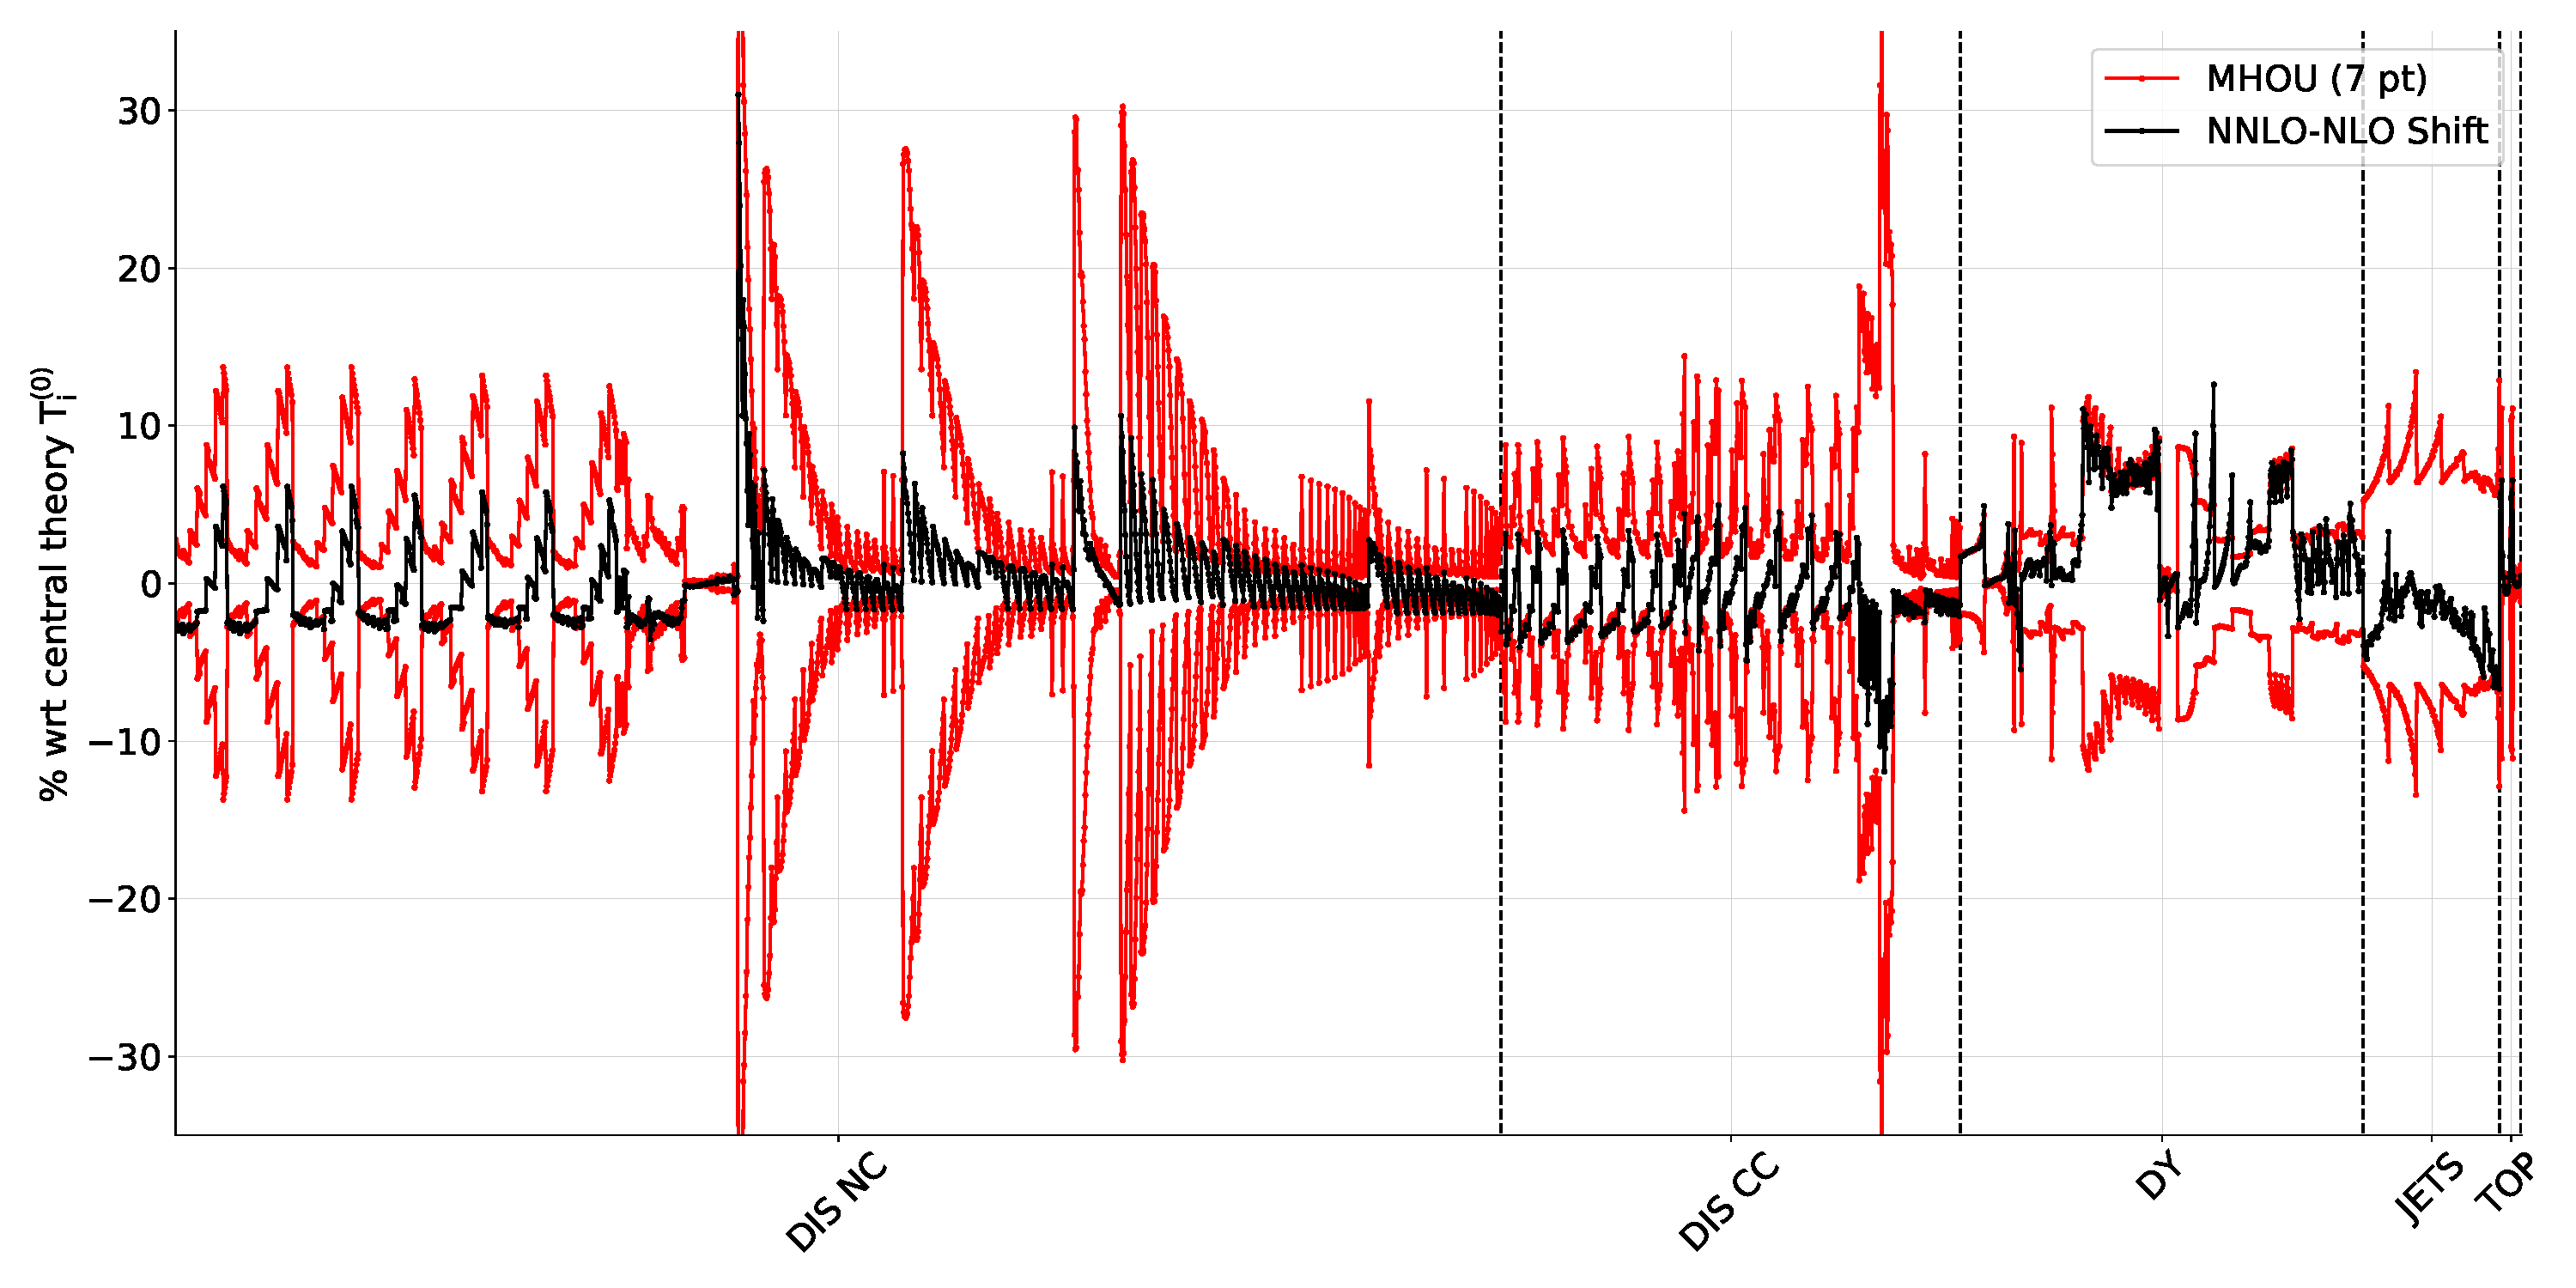
\includegraphics[width=0.69\textwidth]{figures/shift_diag_cov_comparison_7pt_global.pdf}
    \caption*{{\color{gray}\small [NNPDF: 1906.10698]}}
  \end{figure}
\end{frame}

\begin{frame}{Impact of MHOU in a PDF fit}
  \begin{figure}
    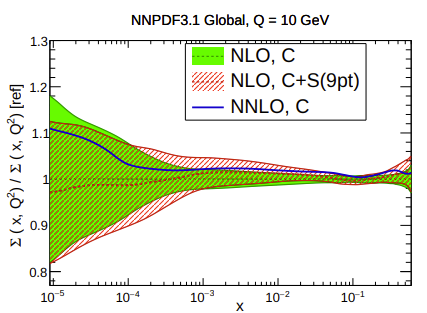
\includegraphics[width=0.49\textwidth]{figures/nnpdf31mhousinglet.png}
    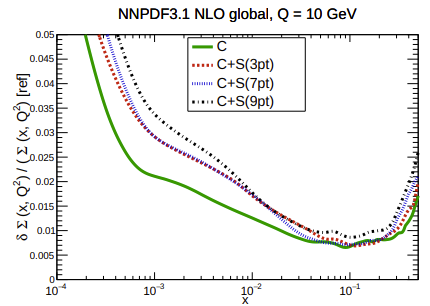
\includegraphics[width=0.49\textwidth]{figures/nnpdf31mhouuncs.png}
  \end{figure}
  Small increase in PDF unceratinty \\
  Soon: NNPDF4.0 with MHOU
\end{frame}

% \begin{frame}{Impact of MHOU on Pheno}
% \end{frame}

% ========================================QED===================================
\section{QED effects in PDFs}

\begin{frame}{Including QED corrections in a PDF set}
  The current standard for PDFs determination is at NNLO in QCD, however  $\alpha(M_z) \sim \alpha_s^2(M_Z)$

  \begin{columns}
    \begin{column}{0.49\textwidth}

      \vspace*{1em}
      Including QED corrections in PDFs consists of \vspace*{0.5em}
      \begin{itemize}
        \item QED corrections to DGLAP (at $\mathcal{O}(\alpha)$, $\mathcal{O}(\alpha \alpha_s)$ and $\mathcal{O}(\alpha^2))$: \\ 
        $P_{QED}=\alpha P_{ij}^{(0,1)}+\alpha \alpha_s P_{ij}^{(1,1)}+\alpha^2 P_{ij}^{(0,2)}+\ldots$
        \vspace*{0.5em}
        \item Adding a photon PDF and including photon initiated contributions to cross-sections \\
        The momenum sumrule is modified accordingly:   
        \begin{equation*}
          \int_0^1 dx\, \left(  x\Sigma(x,Q^2) + xg(x,Q^2) + x\gamma(x,Q^2) \right) =1
        \end{equation*}
      \end{itemize}
    \end{column}

    \begin{column}{0.49\textwidth}
      \begin{figure}
        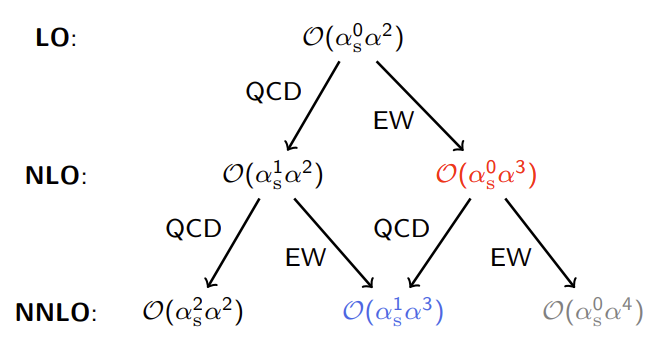
\includegraphics[width=0.99\textwidth]{figures/ewcorrections_dy.png}
        \caption*{Example: EW corrections in DY\\ {\color{gray}\small [C. Schwan DIS 2021]}}
      \end{figure}
    \end{column}
  \end{columns}
\end{frame}


\begin{frame}{Determination of the photon PDF}
  \begin{columns}[T]
    \begin{column}{0.59\textwidth}
      Initially the photon PDF has been determined in different ways:
      \begin{itemize}
        \item physical model: sensitive to underlying model
        \item fitting: data does not provide strong constraints
      \end{itemize}

      \vspace*{0.5em}
      However with the LUXqed approach it can be computed perturbatively \\ 
      based on the observation that the heavy-lepton production cross-section can be written in two ways:
      \begin{itemize}
        \item in terms of structure functions $F_2$, $F_L$
        \item in terms of PDFs including the photon
      \end{itemize}

      \vspace*{0.5em}
      luxQED result {\color{gray}\small[Manohar, Nason, Salam, Zanderighi: 1607.04266, 1708.01256]}:
      \begin{equation*}
        \begin{split}
          & x \gamma(x, \mu^2)
          =
          \frac{2}{\alpha (\mu^2)} \int\limits_x^1 \frac{dz}{z}
          \Biggl\{ \int_{m_p^2x^2 \over 1-z}^{\mu^2 \over 1-z} \frac{dQ^2}{Q^2}
          \alpha^2(Q^2) \Biggl[ -z^2 F_L(x/z, Q^2) \\
          & + \left( z P_{\gamma q}(z) + \frac{2 x^2 m_p^2}{Q^2} \right)
          F_2(x/z, Q^2)\Biggr] - \alpha^2(\mu^2) z^2 F_2(x/z, \mu^2)\Biggr\}
        \end{split}
      \end{equation*}
    \end{column}

    \begin{column}{0.39\textwidth}
      \vspace*{-5em}
      \begin{figure}
        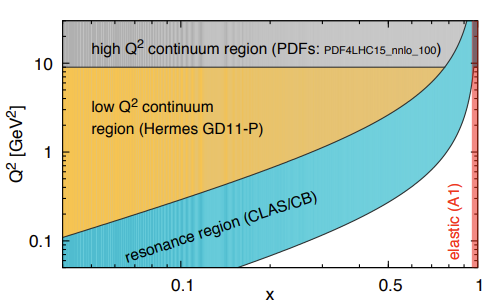
\includegraphics[width=0.89\textwidth]{figures/dataluxqed.png}
        \caption*{Input to construct $F_2$ and $F_L$}
        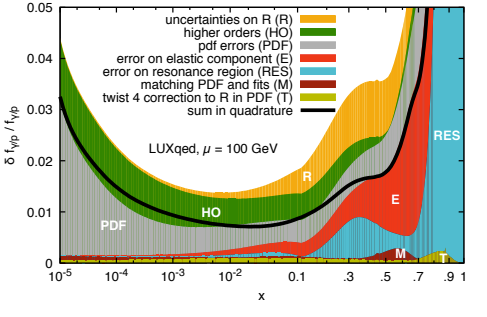
\includegraphics[width=0.89\textwidth]{figures/luxQED_uncs.png}
        \caption*{Sources of unceratinty}
      \end{figure}
    \end{column}
  \end{columns}
\end{frame}


\begin{frame}{LUXqed PDF determinations}
  LUXqed has been used in all of the most recent QED PDFs:
  \begin{itemize}
      \item LUXqed\_plus\_PDF4LHC15 {\color{gray}\small [Manohar, et al.: 1607.04266]}
      \item LUXqed17\_plus\_PDF4LHC15 {\color{gray}\small [Manohar, et al.: 1708.01256]}
      \item MMHT2015qed {\color{gray}\small [Harland-Land et al.: 1907.02750]}
      \item NNPDF3.1luxQED {\color{gray}\small [Bertone et al.: 1712.07053]}
      \item CT18lux and CT18qed {\color{gray}\small [Xie et al.: 2106.10299]}
      \item MSHT20QED {\color{gray}\small [Cridge et al.: 2111.05357]}
      \item Soon: NNPDF4.0QED
  \end{itemize}
\end{frame}

\begin{frame}{The photon PDF by different groups}
  \begin{columns}[T]
    \begin{column}{0.59\textwidth}
      % Details of the, implementation and correspondingly the above equation, vary between PDF fitting groups

      % \vspace*{1em}
      % The input scale $\mu$:
      % \begin{itemize}
      %   \item 1 GeV for MSHT20QED
      %   \item 3(1.3) GeV for CT18qed(1.3GeV)
      %   \item No evolution or sumrule for CT18lux
      %   \item 100 GeV for NNPDF3.1luxQED and NNPDF4.0QED
      % \end{itemize}

      Differences between the studies by the different groups include:

      \vspace*{1em}
      CT18qed initializes the photon at an input scale and evolves using DGLAP, while CT18lux calculates the photon at all scales\\

      \vspace*{0.5em}
      CT18lux performs systematic study of variations to estimate the uncertainty

      \vspace*{1em}
      MSHT20QED has a 1~GeV input scale and includes renormalon corrections

      \vspace*{1em}
      NNPDF follow the original luxQED by calculating the photon at 100~GeV to reduce higher twist effects
      \vspace*{0.5em}
      NNPDF3.1QED and NNPDF4.0QED use an iterative procedure to address the interplay between the photon and other PDFs due to the momentum sumrule
      \begin{equation*}
        \int_0^1 dx\, \left(  x\Sigma(x,Q^2) + xg(x,Q^2) + x\gamma(x,Q^2) \right) =1
      \end{equation*}
    \end{column}

    \begin{column}{0.39\textwidth}
      \vspace*{-1.5em}
      \begin{figure}
        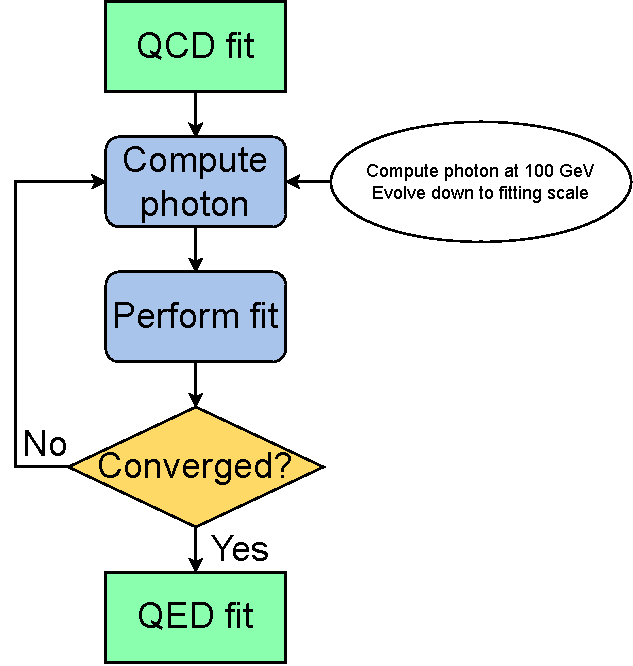
\includegraphics[width=0.9\textwidth]{figures/luxqed_iteration.pdf}
        \caption*{\color{gray}\small [NNPDF3.1QED: 1712.07053]}
      \end{figure}
    \end{column}
  \end{columns}

\end{frame}


\begin{frame}{Impact of the photon on other PDFs}
  \begin{center}
    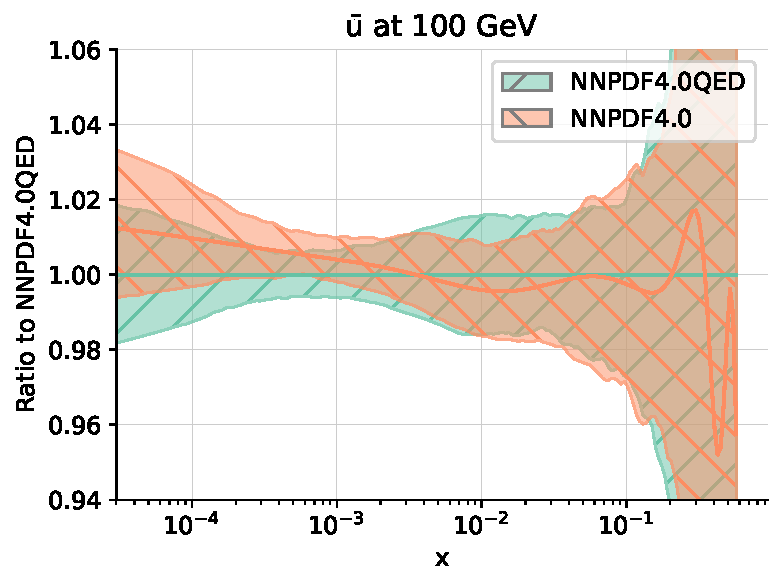
\includegraphics[width=0.45\textwidth]{figures/nnpdf40_vs_qed_ubar.pdf}
    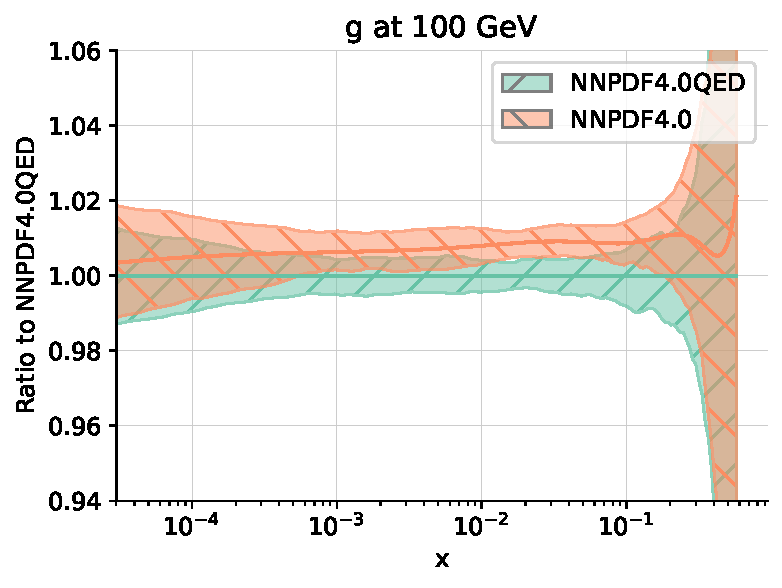
\includegraphics[width=0.45\textwidth]{figures/nnpdf40_vs_qed_g.pdf}
  \end{center}
  \begin{itemize}
    \item PDFs are in agreement within uncertainty
    \item Gluon reduced due to momentum sum rule with photon carrying additional momentum
  \end{itemize}
\end{frame}


\begin{frame}{Results: photon PDF and luminosity}
  \begin{center}
    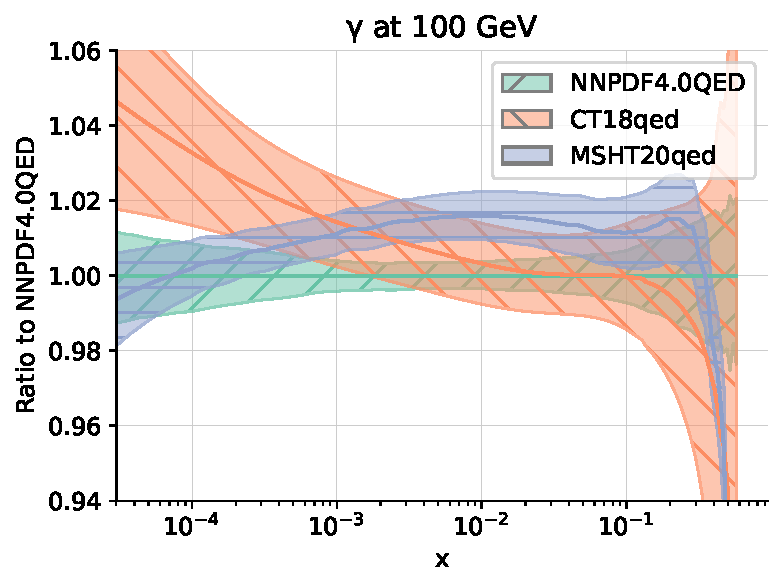
\includegraphics[width=0.3\textwidth]{figures/photon_comparison.pdf}
    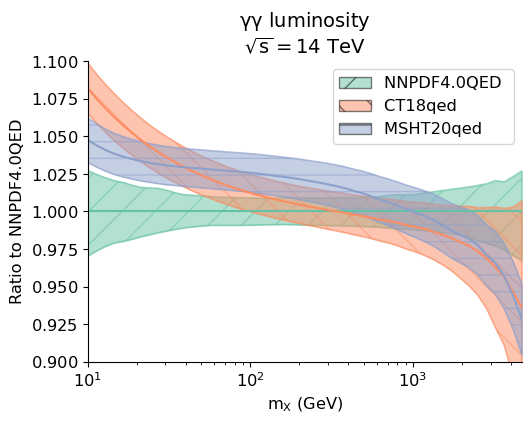
\includegraphics[width=0.3\textwidth]{figures/pp_lumi_comparison.png}
    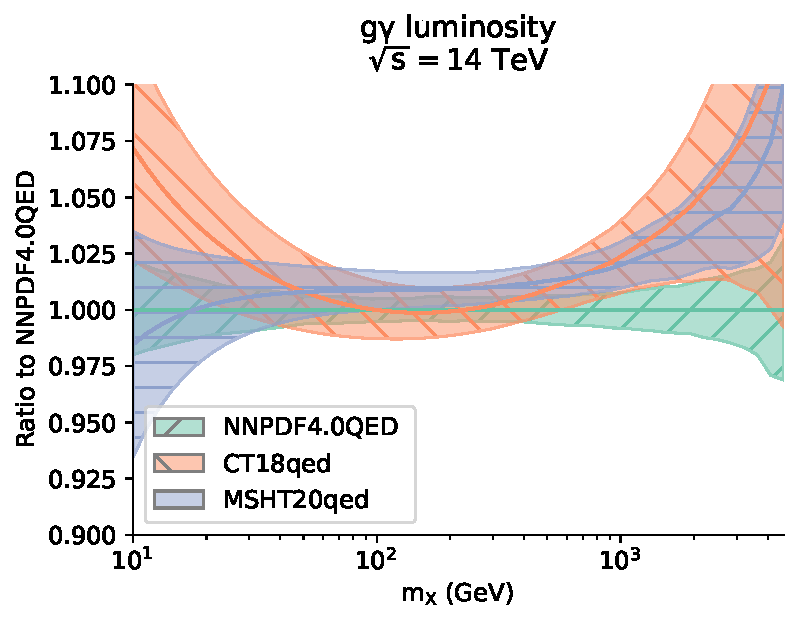
\includegraphics[width=0.3\textwidth]{figures/gp_lumi_comparison.pdf}
  \end{center}
  \begin{itemize}
    \item Because all groups use the luxQED formalism, the photon PDFs agree at percent level
    \item Luminosity generally in agreement, but differ at very small and very large invariant mass
  \end{itemize}
\end{frame}


\begin{frame}{Phenomenological impact of QED effects}
  \begin{columns}[T]
    \begin{column}{0.49\textwidth}
      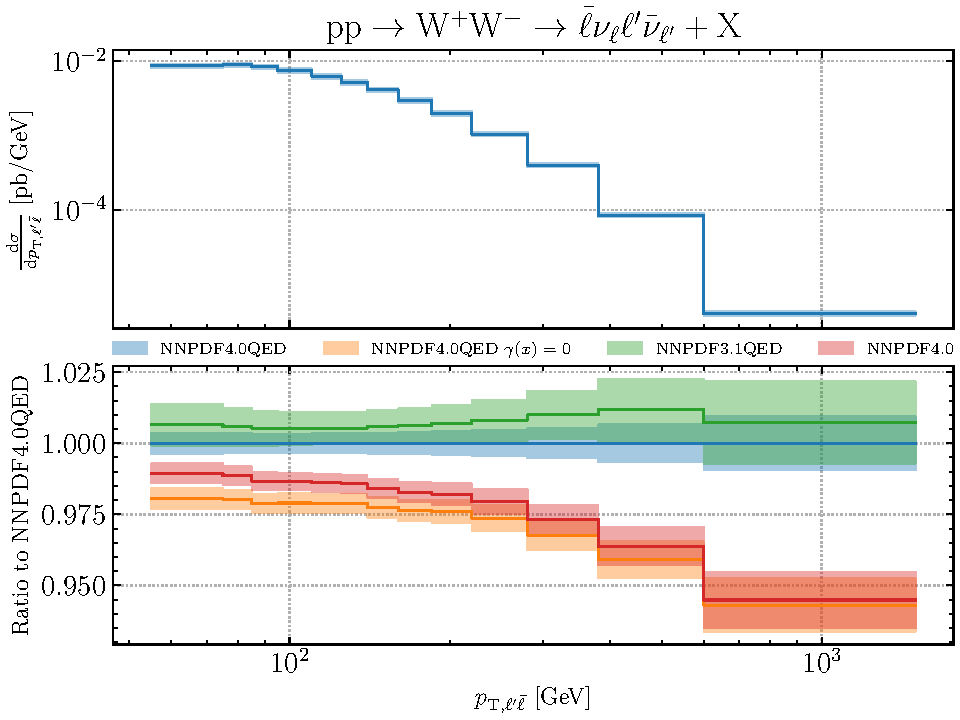
\includegraphics[width=0.7\textwidth]{figures/NNPDF_WPWM_14TEV_40_PHENO-internal.pdf}
    \end{column}
    \begin{column}{0.49\textwidth}
      \vspace*{-3.5em}
      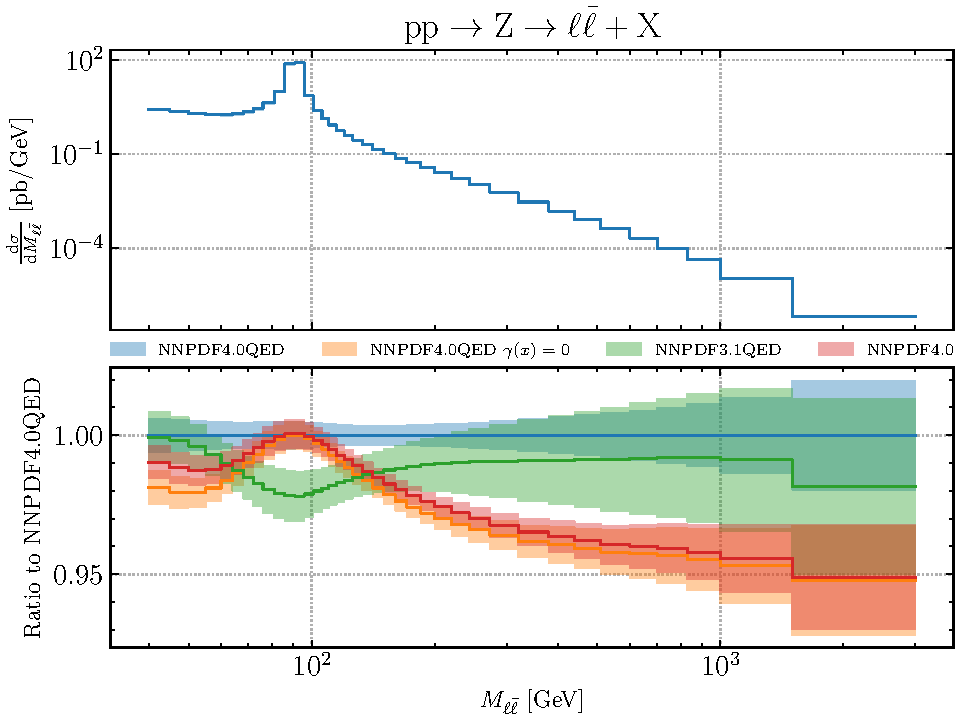
\includegraphics[width=0.7\textwidth]{figures/NNPDF_DY_14TEV_40_PHENO-internal.pdf}
    \end{column}
  \end{columns}
  \begin{columns}[T]
    \begin{column}{0.49\textwidth}
      \vspace*{1em}
      \begin{itemize}
        \item Here photon initiated contributions are included
        \item Non-negligable QED corrections in the large invariant mass and large-$p_T$ regions relevant for new physics searches
        \item Negligable impact around the $Z$-peak
        \item Difference between groups driven by gluon and quark PDFs
        % \item Results produced using PineAPPL grids
      \end{itemize}
    \end{column}
    \begin{column}{0.49\textwidth}
      \vspace*{-3em}
      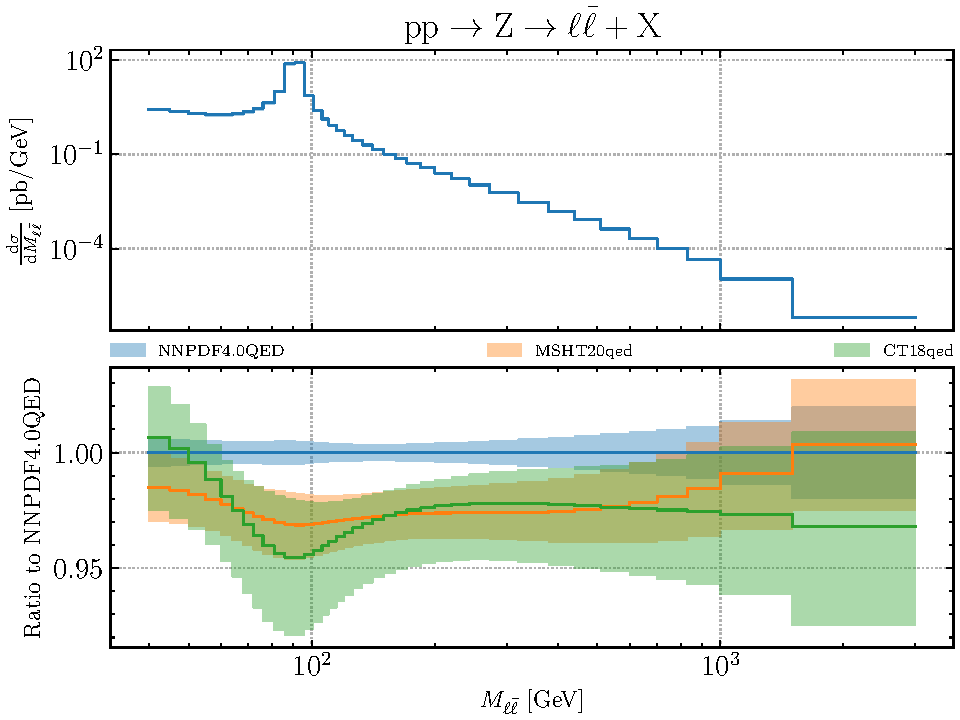
\includegraphics[width=0.7\textwidth]{figures/NNPDF_DY_14TEV_40_PHENO-global.pdf}
    \end{column}
  \end{columns}
\end{frame}


\begin{frame}{PineAPPL: combined QCD and QED interpolation tables}

  PineAPPL is a library for storing PDF-independent theory predictions in interpolation grids\\ {\color{gray}\small [Carazza, Nocera, Schwan, Zaro: 2008.12789 ]}
  \vspace*{1em}

  \begin{columns}
    \begin{column}{0.49\textwidth}
      Typical setup:
      \begin{figure}
        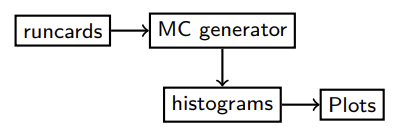
\includegraphics[width=0.5\textwidth]{figures/typicalsetup.png}
      \end{figure}
      Requires rerunning MC generator for each PDF
    \end{column}
    \begin{column}{0.49\textwidth}
      PineAPPL:
      \begin{figure}
        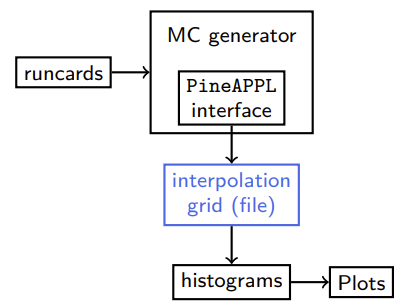
\includegraphics[width=0.5\textwidth]{figures/pineapplsetup.png}
      \end{figure}
      After computing the interpolation grid once it can be convolved with an arbitrary PDF set
    \end{column}
  \end{columns}
  \vfill\hfill{\color{gray}\small [C. Schwan DIS 2021]}
\end{frame}


\begin{frame}{PineAPPL: combined QCD and QED interpolation tables}
  Applications:
  \begin{itemize}
    \item PDF fits
    \item Efficient study of PDF impact on observable (e.g. for SM parameter extraction)
  \end{itemize}

  \vspace*{1em}
  Other providers of fast interpolation grids:
  \begin{itemize}
    \item APPLgrid {\color{gray}\small [Carli et al.: 0911.2985]}
    \item fastNLO {\color{gray}\small [Kluge, Rabbertz, Wobisch: hep-ph/0609285]}
  \end{itemize} 

  However, the need for EW corrections inspired the creation of PineAPPL
  
  \vspace*{1em}
  Finally, PineAPPL...
  \begin{itemize}
    \item supports up to any power in $\alpha$ and $\alpha_s$
    \item is interfaced to MG5\_aMC@NLO
    \item is interfaced to xFitter
    \item is open source
  \end{itemize}
\end{frame}



% ===============================Summary and outlook============================
\section{Summary and outlook}

\begin{frame}{Summary and outlook}

  \begin{columns}[T]
    \begin{column}{0.49\textwidth}
      \vspace*{1em}
      Interpretation of collider measurements depends on accurate and precise theory predictions
    
      \vspace*{1em}
      The last years have seen impressive progress in N3LO calculations for LHC processes, to exploit this we need N3LO PDFs
    
      \vspace*{1em}
      Electroweak effects can no longer be neglected thus include QED corrections in DGLAP and include a photon PDF
    
      \vspace*{1em}
      The target of faithful 1\% uncertainty in wide kinematic range will require simultaneously including EW effects, MHOU, and N3LO!    
    \end{column}
    \begin{column}{0.49\textwidth}
      \begin{figure}
        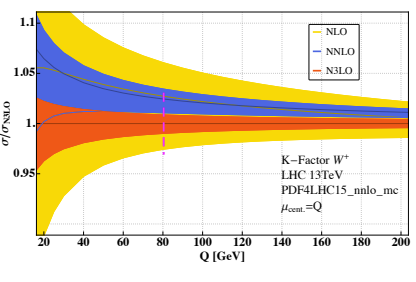
\includegraphics[width=0.9\textwidth]{figures/n3lomistlberger.png}
        \caption*{\color{gray}\small [Duhr, Dulat, Mistleberger 2007.13313]}
      \end{figure}
    \end{column}
  \end{columns}

  \vspace*{2em}
  \only<2>{
  \begin{center}
      {\Large \textbf{Thank you for listening!}}
  \end{center}
  }
\end{frame}


\end{document}
